\documentclass[twoside,11pt,a4paper]{article}

% packages %%%%%%%%%%%%%%%%%%%%%%%%%%%%%%%%%%%%%%%%%%%%%%%%%%%%%%%%%%%%%%%%%%%%
\usepackage{graphicx,curves,float,rotating}


\usepackage{amsmath, amssymb, latexsym}  % math stuff
\usepackage{amsfonts}
\usepackage{amsopn}                             % um mathe operatoren zu deklarieren
\usepackage[american]{babel}                     % otherwise use british or american
\usepackage{theorem}                            % instead of \usepackage{amsthm}
\usepackage{dcolumn}
\usepackage{hyperref}
\usepackage[utf8x]{inputenc}
\usepackage{tikz}
\usepackage{algpseudocode}
\usepackage{algorithm}
\usepackage{subcaption}
\usepackage{tabu}
\usepackage{arydshln} % for dashed vertical line in tabular env
\usepackage[subpreambles=true]{standalone}
\usepackage{hyperref}
\usepackage{todonotes}


\newcommand*\Let[2]{\State #1 $\gets$ #2}



% @ environment %%%%%%%%%%%%%%%%%%%%%%%%%%%%%%%%%%%%%%%%%%%%%%%%%%%%%%%%%%%%%%%%
\usepackage{xspace}                             % context sensitive space after macros
\makeatletter
\DeclareRobustCommand\onedot{\futurelet\@let@token\@onedot}
\def\@onedot{\ifx\@let@token.\else.\null\fi\xspace}
\def\eg{{e.g}\onedot} \def\Eg{{E.g}\onedot}
\def\ie{{i.e}\onedot} \def\Ie{{I.e}\onedot}
\def\cf{{c.f}\onedot} \def\Cf{{C.f}\onedot}
\def\etc{{etc}\onedot} \def\vs{{vs}\onedot}
\def\wrt{w.r.t\onedot} \def\dof{d.o.f\onedot}
\def\etal{{et al}\onedot}
\def\zB{z.B\onedot} \def\ZB{Z.B\onedot}
\def\dh{d.h\onedot} \def\Dh{D.h\onedot}
% %%%%%%%%%%%%%%%%%%%%%%%%%%%%%%%%%%%%%%%%%%%%%%%%%%%%%%%%%%%%%%%%%%%%%%%%%%%%%%%



%%%%%%%%%%%%%%%%%%%%%%%%%%%%%%%%%%%%%%%%%%%%%%%%%%%%%%%%%%%%%%%%%%%%%%%%%%%%%%%
%
%
%	Macros fuer neue Umgebungen
%
%
%%%%%%%%%%%%%%%%%%%%%%%%%%%%%%%%%%%%%%%%%%%%%%%%%%%%%%%%%%%%%%%%%%%%%%%%%%%%%%%
\newcommand*{\Frac}[2]{\frac{\displaystyle #1}{\displaystyle #2}}
\newlength{\textwd}
\newlength{\oddsidemargintmp}
\newlength{\evensidemargintmp}
\newcommand*{\hspaceof}[2]{\settowidth{\textwd}{#1}\mbox{\hspace{#2\textwd}}}
\newlength{\textht}
\newcommand*{\vspaceof}[3]{\settoheight{\textht}{#1}\mbox{\raisebox{#2\textht}{#3}}}
\newcommand*{\PreserveBackslash}[1]{\let\temp=\\#1\let\\=\temp}

\newenvironment{deflist}[1][\quad]%
{  \begin{list}{}{%
      \renewcommand{\makelabel}[1]{\textbf{##1}\hfil}%
      \settowidth{\labelwidth}{\textbf{#1}}%
      \setlength{\leftmargin}{\labelwidth}
      \addtolength{\leftmargin}{\labelsep}}}
{  \end{list}}


\newenvironment{Quote}% Definition of Quote
{  \begin{list}{}{%
      \setlength{\rightmargin}{0pt}}
      \item[]\ignorespaces}
{\unskip\end{list}}


\theoremstyle{break}
\theorembodyfont{\itshape}
\theoremheaderfont{\scshape}

\newtheorem{Cor}{Corollary}
\newtheorem{Def}{Definition}
%\newtheorem{Def}[Cor]{Definition}



\newcolumntype{.}{D{.}{.}{-1}}


\pagestyle{headings}
\textwidth 15cm
\textheight 23cm
\oddsidemargin 1cm
\evensidemargin 0cm
%\parindent 0mm



\begin{document}


\pagestyle{empty}

\begin{center}

    RWTH Aachen University\\
    Chair of Computer Science 6 \\
    Prof. Dr.-Ing. Hermann Ney\\[6ex]
    Selected Topics in Human Language Technology and Pattern Recognition WS 16/17\\[12ex]

    \LARGE
    \textbf{Deep Directed Generative Models} \\[6ex]
    \textit{André Merboldt} \\[6ex]
    \textit{346703} \\[6ex]
    \today

    \vfill
    \Large Supervisor: Tobias Menne
\end{center}

% blank page
\newpage
\
\newpage


% contents
\pagestyle{headings}
\tableofcontents
\listoftables
\listoffigures
%\newpage
%\pagestyle{empty}
%\
\newpage
\pagestyle{headings}


%----------------------------------
% ABSTRACT
%----------------------------------
\section{Abstract}
\label{sec:abstract}
Deep Learning has advanced at an incredible speed the last few years and has achieved human-level performance in some discrimination and classification tasks (object recognition, speech recognition).
These supervised methods have the huge drawback of requiring a vast amount of labeled data which is often expensive or unfeasible to obtain.
Learning hidden structure from unlabelled data known as unsupervised learning has had less of an impact recently.
However, it can be argued that this learning is most similar to human learning, in particular inferring information from observations and building an appropriate model from it.
We will discuss and explore some models for performing aforementioned inference as well as generating new data from these representations.
Building reasonable representation of the world from unlabelled data is arguably one of the key aspects to machine intelligence.
%However one of the key aspects to machine intelligence is learning a rich (?) model about the world and draw conclusions from it.
%The above mentioned tasks require huge amount of labelled data to perform well, which is one of the restrictions of these supervised learning mechanisms.
%Unsupervised learning has the potential to make use of the vast unlabelled data surrounding the world.
%This data can be used to learn representations 


%In this seminar paper we provide an overview and introduction to directed generative models,
%which are able to produce data following a distribution (...?).
% more info what generative models try to achieve
%After we have introduced several architectures, we will explore sigmoid belief networks (SBN)
%as an early generative model.\\

%Then we will turn to more recent proposals, in particular variational autoencoders (VAE) and
%generative adversarial networks (GAN).
%Variants of GANs have been shown to produce images which are able to fool a human discriminator 40\% of the time (citation needed, LAPGAN? or DCGAN?).
%Additionally to exploring these models and theoretical foundation, we provide an intuitive and simple application of a GAN.







%----------------------------------
% Motivation
%----------------------------------
\section{Introduction}
\label{sec:introduction}

"What I cannot create, I do not understand." -- Richard Feynman \\\\\\



Directed generative models are a wide class of models used for generating samples from an unknown distribution.
Lets denote $p_{data}(x)$ as the real-world data distribution which is unknown, however we have access to samples from it: $x \sim p_{data}(x)$.
In order to do so, we define an approximated distribution $p_{model}$ from which we are able to sample.
Under the assumption that $p_{model}$ approximates $p_{data}$ accurately, samples from the true data distribution should have high likelihood under the approximation as well.\\\\

Generative modelling has several important application areas, which will be highlighted on below.\\
Deep learning techniques have provided great success in applying gradient-based optimization methods to deep neural networks to achieve impressive results in discriminative models.
These models require however large amounts of labelled data, which is often expensive or infeasible to obtain.
Generative models can be used to learn \emph{representational} structures from rich, unlabelled data by having less parameters than the input data and are thus forced to capture only essential information.\\
\newpage


%Prior to discussion individual models, we need to declare a few assumptions and definitions.
%Additionally we assume that samples $x$ are also conditionally dependent on some hidden structure $z$: $x \sim p(x|z)$. 
%\begin{equation}
  %z \sim p(z)\\
  %x \sim p(x|z)
%\end{equation}

%\paragraph{Sampling}
%means for any given $z$ to draw a sample $x$ from our model.
%Most commonly, sampling is the easiest requirement to fulfil.

%\paragraph{Learning}
%of the model parameters through maximum likelihood estimation generally involves $p(x)$ or its gradient.\\
%To get $p(x)$, we first need to marginalize our the latent variables.
%\begin{equation}
  %p(x) = \sum_h p(x|z)p(z)
%\end{equation}
%Unfortunately, in the case of deep learning with many layers this is intractable, as we need to evaluate all model configurations.
%via maximum likelihood generally involves the gradients of $p(x)$
%\paragraph{Inference}
% motivation / what we want exactly and why
%Building intelligent systems requires having accurate and generalized information about the environment in order to perform actions or reason about the world.
%Inferring structured and meaning information from unlabelled data, a process called unsupervised learning, remains a challenging task.

%However, due to the massive increases in availability of data emerging from the web as well as the ongoing progress in computational power there has been significant progress using this data.

%Generative modelling aims to generate new data similar to previously seen input, in a way which is sound with the internal structure of the data.

%% on building reasonable representations
The assumption that data can be explained using an underlying, simpler structure than the raw input data is important to handle the high-dimensional nature of most data source.
In order to understand how these statistical models help us to discover the data structure, we will take a look at a few examples of high-dimensional real world data.
\begin{itemize}
  \item \textbf{Images} consisting of millions of pixels can be interpreted as data where each pixel represents an own dimension.
  However, these dimensions are high correlated and structured, for example nearby pixels have with high probability similar values.
  Looking at images of handwritten digits, the data can be reduced to a handful variables which may include the digit number, stroke width, position or size.
  Statistical models help us discover these relations and reduce them to representations in lower dimensional space.
  %\item commonly have thousands of dimensions, but the underlying structure is often far simpler. For example are 28x28 images of handwritten digits 784-dimensional but assuming one-hot encoding the most important information - the digit - it can be explained using 10 dimensions. There are a few more dimensions, stroke width, cursive, position, size. But still far lower than 784. We will take a look at this example later on in \ref{sec:vae}.
  \item \textbf{Audio data} is omni-present in the real world, however most data sources can be transformed from raw audio samples to spoken words or musical notes without losing too much information for reconstruction.
  \item \textbf{...}
\end{itemize}
% cope with
%To develop systems learning from real world data we use statistical models which are able to infer the underlying structure from
%Real world data is often high-dimensional and noise and transforming this data into an compact representation is therefore an important and also challenging task to perform.
%Generative models are ideal for this task since it has to understand the underlying structure to generate similar data.
%Building this structure is called \textbf{representation learning} and is key to many generative models and how they perform.\\

%With this assumption in mind we can take a look at some examples of input data.




The assumption that $p(x)$ is dependent on some underlying structure can now be expressed as having the conditional probability $p(x|z)$ where the latent variables $z$ are the causal factors. This stochastic dependency can be represented in a graphical model shown in figure \ref{fig:dgm}.\\

\begin{figure}[htb]
\centering

\includegraphics{media/directed_graphical_model}
  \caption{Directed graphical model}
  \label{fig:dgm}
  \medskip
  \small
  Arrows show stochastic dependency.
\end{figure}

%Inverting $p(x|z)$ yields $p(z|x)$ which is one of the main tasks of some generative models, for example the VAE \ref{sec:vae}.


%After a short overview of different approaches and methods and an introductory example with the sigmoid belief net (SBN), we will take a closer look at two recent promising frameworks, the variational autoencoder (VAE \ref{sec:vae}) and the generative adversarial network (GAN \ref{sec:gan}).



%Generative models are one of the most promising ways to perform unsupervised learning (citation needed).
%More specifically, generative modelling assumes a hidden structure $z$ explaining the input data $x$.
%This assumption is reasonable given the following examples:\\




%Generative models have been proposed as one of the most promising approaches towards
%learning representations of real world data by some of the leading researchers (YannLeCun, OpenAI blogpost).

%In recent years supervised learning has yielded impressive results,
%however for these models to succeed huge amount of labelled data is needed.
%Unsupervised learning, that is learning from unlabelled data, has been expressed
%as one hurdles toward general articial intelligence (citation needed).
%Early approaches toward this problem however have shown that these problems are very hard to learn (intractable?).

%In generative models the approach is different in a way that
%we search for a good internal representation of the data.
%This resembles the way humans learn about the world where we incrementally build
%a model of the world.




%----------------------------------
% Overview of Directed Generative Models
%----------------------------------
%\section{Overview of Directed Generative Models}
\label{sec:overview}


\paragraph{Variational Autoencoders (VAE) \cite{vae:2013}\cite{rezende:2014}}
\label{par:overview_vae}
Variational Autoencoders (VAE) use two networks called encoder and decoder where the encoder transform the given data into a latent space and the decoder translates this latent space back into the data space.
The input and output space are usually high-dimensional data spaces, for example images while the latent space is low-dimensional in comparison.
Like other autoencoders, VAEs try to reconstruct the input data using the latent variables as closely as possible.
But in addition to regular autoencoders encourages the VAE the latent space to match a specific probability distribution.
This encouragement is done using a variational lower bound on the distribution output by the encoder network.

%where the encoder takes input data and translates it into a latent structure while
%the decoder takes the latent structure and produces data which is as close as possible to the initial input data.

%In the case of VAEs, the distribution is intractable and we can only approximate the posterior distribution.
% intractable -> use neural network, which we can train
% --> no closed form possible
%We use the KL-Divergence to train the network.

% TODO read chapter 19, approximate inference
%In VAEs however, this 




\paragraph{Generative Adversarial Networks}
\label{par:overview_gan}
GANs are a game theoretic approach to generative modelling
in which two networks compete against each other.
The discriminator $D$ is trying to distinguish the generated samples
by the generator $G$ from real world data.
The goal for $G$ however is to produce data as realistic as possible.\\
During the early phase of training, $G$ produces random noise which
is easy to differentiate from groundtruth data.
Both networks are trained in parallel, where both networks try to get better
at their respective objective.
In the best-case scenario is $G$ able to produce data indistinguishly from real world data in which
case the discriminator will only be able to guess correctly with a 50\% chance.
This plateau is called Nash equilibrium (citation needed).








%----------------------------------
% Sigmoid Belief Networks
%----------------------------------
\section{Sigmoid Belief Networks}
\label{sec:sbn}
\begin{figure}[htb]
\centering
%& /home/spotlight/.config/TikzEdtWForms/TikzEdtWForms/0.2.1.0/temp_header
\documentclass{standalone}
\usepackage{pgfplots}
\pgfplotsset{compat=1.12}

\begin{document}
\usetikzlibrary{arrows.meta,calc,fit}
\usetikzlibrary{backgrounds}
\tikzstyle{h_unit} = [circle, draw, fill=blue!20, node distance=3cm, text width=2.5em, text centered]
\tikzstyle{h_text} = [rectangle, fill=blue!20, text centered]
\tikzstyle{o_unit} = [circle, draw, fill=red!20, node distance=3cm, text width=2.5em, text centered]
\tikzstyle{o_text} = [rectangle, fill=red!20, text centered]

\tikzstyle{arr} = [thick,-{Latex[length=3mm,width=3mm]}]
\begin{tikzpicture}


% first hidden layer
\node [h_unit] (hidden_l1_1) {};
\node [h_unit] (hidden_l1_2) at ([shift={(2,0)}] hidden_l1_1) {};
\node (hidden_l1_others) at ([shift={(1,0)}] hidden_l1_1) {\Large $\cdots$};

% second hidden layer
\node [h_unit] (hidden_l2_1) at ([shift={(-1.5,-2)}] hidden_l1_1){};
\node [h_unit] (hidden_l2_2) at ([shift={(1,-2)}] hidden_l1_1) {};
\node [h_unit] (hidden_l2_3) at ([shift={(3.5,-2)}] hidden_l1_1) {};
\node (hidden_l2_others_1) at ([shift={(1.25,0)}] hidden_l2_1) {\Large $\cdots$};
\node (hidden_l2_others_2) at ([shift={(1.25,0)}] hidden_l2_2) {\Large $\cdots$};

% "stochastic hidden causes"
\node [h_text] (text_hidden) at ([shift={(1,1)}] hidden_l1_1) {\Large hidden causes};

% observable layer
\node [o_unit] (observed_1) at ([shift={(-1,-4)}] hidden_l1_1){};
\node [o_unit] (observed_2) at ([shift={(4,0)}] observed_1) {};
\node (observed_others) at ([shift={(2,0)}] observed_1) {\Large $\cdots$};

% "observed variables"
\node [o_text] (text_observed) at ([shift={(1,-5)}] hidden_l1_1) {\Large observed variables};

% layer backgrounds:
% We are not showing the layer boundaries for now,
% because in the initial sigmoid belief nets there was no
% notion of layers (just ancestors)
\begin{pgfonlayer}{background}
  \node[] () {};
% \node[
%       fill=black!20,
%       node distance=4cm,
%       inner sep = 1em,
%       fit=(hidden_l1_1) (hidden_l1_2)
%       ] (layer_1){};
% 
% \node[
%       fill=black!20,
%       node distance=4cm,
%       inner sep = 1em,
%       fit=(hidden_l2_1) (hidden_l2_2) (hidden_l2_3)
%       ] (layer_2){};
\end{pgfonlayer}

% arrows from first hidden unit in first "layer"
\draw[arr] (hidden_l1_1) -- (hidden_l2_1);
\draw[arr] (hidden_l1_1) -- (hidden_l2_2);
\draw[arr,dashed] (hidden_l1_1) -- (observed_1);

% arrows from second hidden unit in first "layer"
\draw[arr] (hidden_l1_2) -- (hidden_l2_2);
\draw[arr] (hidden_l1_2) -- (hidden_l2_3);

% arrows from first hidden unit in second "layer"
\draw[arr] (hidden_l2_1) -- (observed_1);

% arrows from second hidden unit in second "layer"
\draw[arr] (hidden_l2_2) -- (observed_1);
\draw[arr] (hidden_l2_2) -- (observed_2);

% arrows from third hidden unit in second "layer"
\draw[arr] (hidden_l2_3) -- (observed_2);
\end{tikzpicture}
\end{document}

  \caption[Architecture of Sigmoid Belief Nets]{Conceptual architecture of belief nets}
  \label{fig:sbn_arch}
  \medskip
  \small
  Bayesian networks, also called belief nets are an acyclic directed graph where blue nodes indicate hidden variables and red nodes represent observed variables.
  Arrows indicate stochastic dependency.
  Even though most belief nets are divided into many layers in the context of deep learning, the original definition does not specify that and thus indicates the dashed arrow the possibility of inter-layer dependencies.
\end{figure}

Sigmoid Belief Networks (SBN) were described in 1992 by R.M. Neal \cite{neal:1992} representing a specific type of bayesian networks \cite{pearl:1985} shown in Figure \ref{fig:sbn_arch}
In the case of SBNs however, all states are binary and the activation function is the sigmoid function. They are one of the earliest neural networks used for generative modeling, predating all other presented models in this article.
%As described in the overview above, SBNs contain a number of binary states $s$, most commonly divided into many layers.
Each state $s_i$ is a random variable in the bayesian framework which means it can be observed, hidden or unknown representing different states of knowledge. As such it can also be interpreted with a probability distribution.
\begin{equation}
  \label{eq:sbn_node}
p(s_i) = \sigma\bigg(\sum_{j<i}W_{j,i}s_j+b_i\bigg)
\end{equation}
where 
\begin{conditions}
  \sigma(x) & $\frac{1}{1 + e^{-x}}$ (sigmoid function)\\
  W_{j,i} & connection weights from state $s_j$ to $s_i$\\
\end{conditions}

To draw samples from this network, it is possible to simply evaluate Equation~\ref{eq:sbn_node} for each visible node.
However prior to that, the SBN first needs to learn how to generate good samples which includes the \emph{learning} and the \emph{inference} problem.\\
Learning means in this context to adjust the weights and biases of the network to be more likely to generate data similar to samples from the given training dataset.
Meanwhile statistical inference is tasked to infer the states of the hidden nodes based on the states in the visible layer.\\

Due to each state being statistically depend on all ancestors, inference means to evaluate all possible configurations of every previous node.
Especially in deep networks, this kind of computation is infeasible as it requires computing exponentially many configurations.\\

% TODO: connection to DBN, layer-wise greedy training
% Hinton et al. (2006)

% DONE

%However in order to draw good samples from this network, the weights need to be adjusted to make it 
%However most other operations involving this network are intractable for most cases, like learning and performing inference.

%In probabilistic networks, we are mostly interested in the aspects: sampling, learning and inferring.
%Even though sampling can be done efficiently, the other operations are intractable in almost all cases.
%\paragraph{Sampling}
%can be done using ancestral sampling through the hidden layers evaluating \ref{eq:sbn_node}

%These random variables are interpreted in a bayesian way where each one may be observed, hidden (or latent) or unknown representing different states of knowledge or belief \cite{definetti:1974}.

%\newpage
%\subsection{Learning}
%\begin{figure}[htb]
%\centering
%\includestandalone[mode=buildnew]{media/sbn_node}
  %\caption{SBN node}
  %\label{fig:sbn_node}
%\end{figure}


%In its most common form, SBNs are comprised by a number of layers where each node in a layer is a sigmoid function of its ancestors:

%While sampling from these networks is very efficient, computing the inference $p(z|x)$ over the hidden units is intractable.
%% show why?

%There have been several attempts on solving the inference problem, using inference networks which have shown promising results.

\newpage


%----------------------------------
% Variational Autoencoders
%----------------------------------
\section{Variational Autoencoders}
\label{sec:vae}
Variational Autoencoders (VAE) have been introduced in 2014 by Kingma and Welling which uses variational inference to perform efficient inference and learning in deep latent models.
Deep latent models are based on the assumption that input data can be explained using non-linear transformations coming from simple distributions. \cite{rezende:2014} (check!?).

Given this assumption, building a good representation in the latent space is crucial for minimal reconstruction error as well as good generative modelling in practice(?).

\paragraph{Formal Setup}
Formally, $p(x,z)$ is the joint probability distribution over both input and latent variables while $p(z|x)$ is the conditional probability of the latent variables given input data.
Inferring the posterior distribution $p(z|x)$ is particularly interesting, because it means to enable learning parameters for good latent space representation.
$p(z|x)$ can be expanded using bayes rule to $\frac{p(x|z) p(z)}{p(x)}$.
Computing the nominator is straightforward, $p(z)$ is the probability distribution we chose for the latent space, oftenmost simply a gaussian.
$p(x|z)$ is easy to compute as well, ...? (forward pass?).\\
Meanwhile is the denominator difficult to evaluate, because it requires to consider all possible input combinations.
What we do instead in the variational autoencoders is to derive a lower-bound on $p(z|x)$ using a auxiliary distribution called $q_\theta(z|x)$. The subscript $\theta$ indicates that the distribution is parametrized by an variational term, so that for one $\theta$, $q_\theta(z|x) \approxeq p(z|x)$ holds ($q(z|x)$ doesn't need to depend on $x$).
%Performing statistical inference means computing $p(z|x)$ which is intractable in all but very simple cases (integrating over it, show calc).

%In this setup we have observed variables $x$ from which we would like to infer latent variables $z$


%Variational Autoencoders (VAE) have been a popular choice for unsupervised learning of complicated distributions (citation needed) and generative modelling.
%In order to generate data from unknown and mostly intractable distributions, we need approximations.
%There are basically two approaches for sampling from these distributions,
%first there are approximate samples (MCMC, gibbs sampling, etc) which try to directly approximate $p(x)$.
%Variational Autoencoders instead try to match an easier to compute distribution $q(x)$ to $p(x)$.
%By using this approach, VAEs are computationally less intensive (citation?) but have the drawback of being more restricted in their modelling approach.
%Practically, this means that with more computation MCMC methods approach $p(x)$, while there is no such guarantee for variational methods (--> not for all).

%VAE can be learned with just backpropagation (paper,TODO), but they differ from denoising and sparse autoencoders due to the different loss function.


%VAEs are built on top of neural networks and are designed in a way to allow training with gradient-based methods.
%Learning and inference are reasonable efficient and relatively easy to implement and show decent results, but have been overshadowed by more recent adversarial approaches (citation needed!!,see \ref{sec:gan}).

\subsection{Architecture}
\label{sub:vae_architecture}

\begin{figure}[htb]
\centering
\resizebox{5cm}{!}{\definecolor{cdfdfdf}{RGB}{223,223,223}
\definecolor{cffffff}{RGB}{255,255,255}


\begin{tikzpicture}[y=0.80pt, x=0.80pt, yscale=-1.000000, xscale=1.000000, inner sep=0pt, outer sep=0pt]
\begin{scope}[cm={{1.25,0.0,0.0,-1.25,(0.0,1052.3622)}}]
  \begin{scope}[shift={(306.491,697.587)}]
    \path[draw=black,fill=cdfdfdf,line join=miter,line cap=butt,miter
      limit=10.00,nonzero rule,line width=0.319pt] (9.9628,0.0000) .. controls
      (9.9628,5.5023) and (5.5023,9.9628) .. (0.0000,9.9628) .. controls
      (-5.5023,9.9628) and (-9.9628,5.5023) .. (-9.9628,0.0000) .. controls
      (-9.9628,-5.5023) and (-5.5024,-9.9628) .. (0.0000,-9.9628) .. controls
      (5.5023,-9.9628) and (9.9628,-5.5024) .. (9.9628,0.0000) -- cycle;
  \end{scope}
    \path[cm={{1.0,0.0,0.0,-1.0,(303.468,695.373)}},fill=black,nonzero rule]
      (0.0000,0.0000) node[above right] (text4171) {$x$};
  \begin{scope}[shift={(306.491,697.587)}]
    \path[draw=black,fill=cffffff,line join=miter,line cap=butt,miter
      limit=10.00,nonzero rule,line width=0.319pt] (9.9628,48.6708) .. controls
      (9.9628,54.1732) and (5.5024,58.6336) .. (0.0000,58.6336) .. controls
      (-5.5023,58.6336) and (-9.9628,54.1732) .. (-9.9628,48.6708) .. controls
      (-9.9628,43.1685) and (-5.5024,38.7081) .. (0.0000,38.7081) .. controls
      (5.5023,38.7081) and (9.9628,43.1685) .. (9.9628,48.6708) -- cycle;
  \end{scope}
    \path[cm={{1.0,0.0,0.0,-1.0,(303.945,744.043)}},fill=black,nonzero rule]
      (0.0000,0.0000) node[above right] (text4181) {$z$};
    \path[cm={{1.0,0.0,0.0,-1.0,(260.848,741.767)}},fill=black,nonzero rule]
      (0.0000,0.0000) node[above right] (text4187) {$\phi$};
    \path[cm={{1.0,0.0,0.0,-1.0,(345.199,742.798)}},fill=black,nonzero rule]
      (0.0000,0.0000) node[above right] (text4193) {$\theta$};
  \begin{scope}[shift={(306.491,697.587)}]
    \path[draw=black,dash pattern=on 2.39pt off 2.39pt,line join=miter,line
      cap=butt,miter limit=10.00,line width=0.319pt] (-38.5088,48.6708) --
      (-10.9710,48.6708);
  \end{scope}
  \begin{scope}[shift={(295.52,746.258)}]
    \path[draw=black,fill=black,line join=miter,line cap=butt,miter
      limit=10.00,nonzero rule,line width=0.319pt] (-5.2035,2.3356) --
      (0.2989,0.0000) -- (-5.2035,-2.3356) -- (-5.2035,2.3356) -- cycle;
  \end{scope}
  \begin{scope}[shift={(306.491,697.587)}]
    \path[draw=black,line join=miter,line cap=butt,miter limit=10.00,line
      width=0.319pt] (38.5088,48.6708) -- (10.9710,48.6708);
  \end{scope}
  \begin{scope}[cm={{-1.0,0.0,0.0,-1.0,(317.462,746.258)}}]
    \path[draw=black,fill=black,line join=miter,line cap=butt,miter
      limit=10.00,nonzero rule,line width=0.319pt] (-5.2035,2.3356) --
      (0.2989,0.0000) -- (-5.2035,-2.3356) -- (-5.2035,2.3356) -- cycle;
  \end{scope}
  \begin{scope}[shift={(306.491,697.587)}]
    \path[draw=black,line join=miter,line cap=butt,miter limit=10.00,line
      width=0.319pt] (38.5088,45.5084) -- (7.1087,8.4005);
  \end{scope}
  \begin{scope}[cm={{-0.64792,-0.7657,0.7657,-0.64792,(313.6,705.988)}}]
    \path[draw=black,fill=black,line join=miter,line cap=butt,miter
      limit=10.00,nonzero rule,line width=0.319pt] (-5.2035,2.3356) --
      (0.2989,0.0000) -- (-5.2035,-2.3356) -- (-5.2035,2.3356) -- cycle;
  \end{scope}
  \begin{scope}[shift={(306.491,697.587)}]
    \path[draw=black,dash pattern=on 2.39pt off 2.39pt,line join=miter,line
      cap=butt,miter limit=10.00,line width=0.319pt] (-7.1856,7.1856) .. controls
      (-16.6444,16.6438) and (-16.6444,32.0271) .. (-7.7582,40.9132);
  \end{scope}
  \begin{scope}[cm={{0.7071,0.7071,-0.7071,0.7071,(298.733,738.5)}}]
    \path[draw=black,fill=black,line join=miter,line cap=butt,miter
      limit=10.00,nonzero rule,line width=0.319pt] (-5.2035,2.3356) --
      (0.2989,0.0000) -- (-5.2035,-2.3356) -- (-5.2035,2.3356) -- cycle;
  \end{scope}
  \begin{scope}[shift={(306.491,697.587)}]
    \path[draw=black,line join=miter,line cap=butt,miter limit=10.00,line
      width=0.319pt] (0.0000,38.5088) -- (0.0000,10.9710);
  \end{scope}
  \begin{scope}[cm={{0.0,-1.0,1.0,0.0,(306.491,708.558)}}]
    \path[draw=black,fill=black,line join=miter,line cap=butt,miter
      limit=10.00,nonzero rule,line width=0.319pt] (-5.2035,2.3356) --
      (0.2989,0.0000) -- (-5.2035,-2.3356) -- (-5.2035,2.3356) -- cycle;
  \end{scope}
    \path[cm={{1.0,0.0,0.0,-1.0,(308.318,675.918)}},fill=black,nonzero rule]
      (0.0000,0.0000) node[above right] (text4239) {N};
  \begin{scope}[shift={(306.491,697.587)}]
    \path[draw=black,line join=miter,line cap=butt,miter limit=10.00,line
      width=0.319pt] (16.5376,62.3527) -- (-16.5376,62.3527) .. controls
      (-18.7386,62.3527) and (-20.5228,60.5685) .. (-20.5228,58.3676) --
      (-20.5228,-21.2037) .. controls (-20.5228,-23.4046) and (-18.7386,-25.1888) ..
      (-16.5376,-25.1888) -- (16.5376,-25.1888) .. controls (18.7386,-25.1888) and
      (20.5228,-23.4046) .. (20.5228,-21.2037) -- (20.5228,58.3676) .. controls
      (20.5228,60.5685) and (18.7386,62.3527) .. (16.5376,62.3527) -- cycle;
  \end{scope}
\end{scope}

\end{tikzpicture}

}
  \caption{VAE architecture (source: VAE paper)}\label{fig:vae_architecture}
\end{figure}
VAE just like other autoencoders encode the input data into a latent space similar to compression of data and is able to decode a vector of latent variables into output while trying to match the output to the input.
But in contrast to other autoencoders (sparse, denoising), we enforce a specific distribution on the latent space.
This allows to sample from this distribution and generate output which will look similar to the data on which the VAE has been trained.
\ref{fig:vae_architecture}.

\paragraph{Relation to Auto-Encoders}
The Variational autoencoder has the same overall architecture than other autoencoders, for example sparse or denoising autoencoders.
Similar to other autoencoder frameworks VAE provides an encoder as well as a decoder model, but in contrast to other autoencoders both networks are probabilistic. This means that the model described by the VAE framework can be seen as a jointly trained probabilistic encoder and probabilistic decoder.
%One of the main differences is that the VAE framework enforces a specific prior distribution on the latent space, most of the time simply an isotropic gaussian.



\paragraph{The Kullback-Leibler Divergence} (KL divergence) is a measurement for the difference between two probability distributions. $\mathcal{D}_{\mathrm{KL}}(P \| Q)$ can informally described as the amount of information which is lost when using $Q$ to represent $P$.
The KL divergence does not obey the triangle inequality and is also not symmetrical, therefore it does not qualify as a metric.
$\mathcal{D}_{\mathrm{KL}}(P||Q)$ can nevertheless be understood as a measure of the difference between $P$ and $Q$ and is as such used in the VAE to approximate the true posterior distribution.

\subsection{Objective Function}
The objective function of the VAE consists of the reconstruction error and the regularizer.
%$\mathcal{L}$ learns both the encoder as well as the decoder with their respective parameters $\phi$ and $\theta$.
% probabilistic encoder $q_\phi(z|x)$ (produces z values from which x could've been generated)
% probabilistic decoder $p_\theta(x|z)$
We will discuss both terms in detail below following the derivation of the lower variational bound $\mathcal{L}$ and the rewritten objective function.

\paragraph{Derivation of lower bound}
Based on \cite[p.~698]{deeplearning:2016}.
\begin{align*}
  \log p(x)\\
  &= \int_z q_\phi(z|x) \log p(x) dz\\
  &= \int_z q_\phi(z|x) \log \frac{p_\theta(x,z)}{p_\theta(z|x)} dz \tag{Bayes' rule}\\
  &= \int_z q_\phi(z|x) \log\bigg(\frac{p_\theta(z,x)}{q_\phi(z|x)} \frac{q_\phi(z|x)}{p_\theta(z|x)}\bigg) dz \tag{Chain rule}\\
  &= \int_z q_\phi(z|x) \bigg(\log\frac{p_\theta(z,x)}{q_\phi(z|x)} + \log\frac{q_\phi(z|x)}{p_\theta(z|x)}\bigg) dz\\
  &= \int_z q_\phi(z|x) \log \frac{p_\theta(z,x)}{q_\phi(z|x)} dz + \int_z q_\phi(z|x) \log\frac{q_\phi(z|x)}{p_\theta(z|x)} dz\\
  &= \underbrace{\int_z q_\phi(z|x) \log \frac{p_\theta(z,x)}{q_\phi(z|x)} dz}_{= \mathcal{L}}+ \underbrace{\mathcal{D}_{\mathrm{KL}}\big(q_\phi(z|x) \| p_\theta(z|x)\big) dz}_{\geq 0}\\
  &\geq \mathcal{L}\\
\end{align*}

$\mathcal{L}$ is called the evidence lower bound with respect to $\log p(x)$.
We further rewrite $\mathcal{L}$ in order decompose the term into two separate terms, the reconstruction error $\mathcal{L}_{rec}$ and the regularizer $\mathcal{L}_{reg}$.

\begin{align*}
  \mathcal{L}
  &= \int q_\phi(z|x) \log\frac{p_\theta(z,x)}{q_\phi(z|x)} dz\\
  &= \int q_\phi(z|x) \log\frac{p(z) p_\theta(x|z)}{q_\phi(z|x)} \tag{we assume that x is conditionally dependent on z} dz\\
  &= \int q_\phi(z|x) \bigg(\log\frac{p(z)}{q_\phi(z|x)} + \log p_\theta(x|z)\bigg) dz\\
  &= -\int q_\phi(z|x) \log\frac{q_\phi(z|x)}{p(z)} dz + \int q_\phi(z|x) \log p_\theta(x|z) dz\\
  &= -\mathcal{D}_{\mathrm{KL}}\big(q_\phi(z|x) \| p(z)\big) + \int q_\phi(z|x) \log p_\theta(x|z) dz\\
  &= \underbrace{-\mathcal{D}_{\mathrm{KL}}\big(q_\phi(z|x) \| p(z)\big)}_{\mathcal{L}_{reg}} + \underbrace{\mathbb{E}_{z \sim q_\phi(z|x)}\big[ \log p_\theta(x|z)\big]}_{\mathcal{L}_{rec}}\\
  &= \mathcal{L}_{reg} + \mathcal{L}_{rec}
\end{align*}


\paragraph{Regularization term $\mathcal{L}_{reg}$} encourages the model to learn simple representations in latent space, due to the negative Kullback-Leibler (KL) divergence between the learned variational distribution $q_\theta(z|x)$ and the latent space prior distribution $p(z)$.

% move to architecture:
%In the original VAE paper, the unit gaussian distribution with diagonal variance was proposed for $p(z)$ and although there have been multiple proposals (citations, multi-modal etc) for different distributions we will stick with $\mathcal{N}(0,I)$ for the sake of simplicity.
% ---

%For two probability distributions $P$ and $Q$, the KL divergence $\mathcal{D}_{\mathrm{KL}}(P||Q)$ can informally be described as the amount of information which is lost when using $Q$ to represent $P$.

\paragraph{Reconstruction error $\mathcal{L}_{rec}$} measures how well the decoder reconstructs the input data using the latent space $z$.
This error is measures using the negative log-likelihood of the conditional probability distribution $p_\theta(x_i|z)$ where $z$ is sampled from $q_\phi(z | x_i)$.
$\mathcal{L}_{\mathrm{rec}}$ is necessary to force the encoder to produce latent variables which can be used to reconstruct the input data well.




\subsubsection{Reparameterization Trick}
To be able to backpropagate the loss function through the VAE, it has to be differentiable and deterministic.
Because we add noise to the encoding, the gradients can't be computed directly. In order to circumvent this restriction, the so-called "reparameterization trick" is applied.
Instead of drawing $z ~ \mathcal{N}(\mu(x), \Sigma(x))$, we sample an auxiliary variable $\epsilon$ from $\mathcal{N}(0, I)$ which we then transform with equation \ref{eq:rep_trick} into $z$.
\begin{equation}
  \label{eq:rep_trick}
  z = \mu(x) + \Sigma^{1/2}(x)*\epsilon
\end{equation}
This allows us to compute the gradient of the loss function and backpropagate through the entire model and only have the stochastic variable $\epsilon$ as input.\\\\

The core idea of VAEs is to match a distribution $q(x)$ to the desired $p(x)$ by enforcing a lower variational bound on $q(x)$ in a way that it seeks to match $p(x)$.
In contrast to other autoencoders, VAEs behave differently due to this lower bound but they resemble the architecture of traditional autoencoders (sparse, denoising).




We use VAEs when we have a complicated distribution $p_\theta(x,z)$ with unknown latent variables $z$.
The prior distribution $p_\theta(z)$ over the latent structure is a centered isotropic(?) multivariate Gaussian denoted by $\mathcal{N}(z;0, I)$.
The constructed architecture uses an probabilistic encoder $q_\theta(z|x)$ and a probabilistic decoder $p_\theta(x|z)$ in a form of neural networks, in the original paper MLP are used\cite{vae:2013} but there are various extensions (see \ref{sub:vae_extensions}, TODO).
Because the posterior is intractable ($p_\theta(x)$), we instead approximately maximize the lower variational bound $L(\theta,\phi;x)$.\\
\begin{equation}
  \mathcal{L}(\theta,\phi;x) = -D_{KL}(q_\theta(z|x)||p_\theta(z)) + \mathbb{E}_{q_\theta(z|x)}[log_{p_\theta}(x|z)]
\end{equation}




\subsection{Learning}
\label{sub:vae_learning}
In practice, the usual choice for $q_\theta(z|x)$ is the multivariate gaussian distribution.
$$
q_\theta(z|x) = \mathcal{N}(z|\mu(X;\vartheta), \Sigma(X;\vartheta))
$$
Because we assume that $P(z)$ is also a multivariate Gaussian distribution, the KL-divergence can now be computed in closed form as follows\cite{derivations:2007}.
\begin{align*}
  \mathcal{D}_{\mathrm{KL}}\big[Q(z) || P(z|x)\big] &= \mathbb{E}\big[\log \frac{p}{q}\big]\\
  \mathcal{D}_{\mathrm{KL}}\big[\mathcal{N}(\mu_0,\Sigma_0) || \mathcal{N}(\mu_1,\Sigma_1)\big]
  &= \frac{1}{2} \big(\mathrm{tr}\big(\Sigma_1^{-1}\Sigma_0\big) + \big(\big)\big)
\end{align*}


\subsection{Inference}
\label{sub:vae_inference}
\begin{figure}[htb]
\centering
%\resizebox{5cm}{!}{\definecolor{cdfdfdf}{RGB}{223,223,223}
\definecolor{cffffff}{RGB}{255,255,255}


\begin{tikzpicture}[y=0.80pt, x=0.80pt, yscale=-1.000000, xscale=1.000000, inner sep=0pt, outer sep=0pt]
\begin{scope}[cm={{1.25,0.0,0.0,-1.25,(0.0,1052.3622)}}]
  \begin{scope}[shift={(306.491,697.587)}]
    \path[draw=black,fill=cdfdfdf,line join=miter,line cap=butt,miter
      limit=10.00,nonzero rule,line width=0.319pt] (9.9628,0.0000) .. controls
      (9.9628,5.5023) and (5.5023,9.9628) .. (0.0000,9.9628) .. controls
      (-5.5023,9.9628) and (-9.9628,5.5023) .. (-9.9628,0.0000) .. controls
      (-9.9628,-5.5023) and (-5.5024,-9.9628) .. (0.0000,-9.9628) .. controls
      (5.5023,-9.9628) and (9.9628,-5.5024) .. (9.9628,0.0000) -- cycle;
  \end{scope}
    \path[cm={{1.0,0.0,0.0,-1.0,(303.468,695.373)}},fill=black,nonzero rule]
      (0.0000,0.0000) node[above right] (text4171) {$x$};
  \begin{scope}[shift={(306.491,697.587)}]
    \path[draw=black,fill=cffffff,line join=miter,line cap=butt,miter
      limit=10.00,nonzero rule,line width=0.319pt] (9.9628,48.6708) .. controls
      (9.9628,54.1732) and (5.5024,58.6336) .. (0.0000,58.6336) .. controls
      (-5.5023,58.6336) and (-9.9628,54.1732) .. (-9.9628,48.6708) .. controls
      (-9.9628,43.1685) and (-5.5024,38.7081) .. (0.0000,38.7081) .. controls
      (5.5023,38.7081) and (9.9628,43.1685) .. (9.9628,48.6708) -- cycle;
  \end{scope}
    \path[cm={{1.0,0.0,0.0,-1.0,(303.945,744.043)}},fill=black,nonzero rule]
      (0.0000,0.0000) node[above right] (text4181) {$z$};
    \path[cm={{1.0,0.0,0.0,-1.0,(260.848,741.767)}},fill=black,nonzero rule]
      (0.0000,0.0000) node[above right] (text4187) {$\phi$};
    \path[cm={{1.0,0.0,0.0,-1.0,(345.199,742.798)}},fill=black,nonzero rule]
      (0.0000,0.0000) node[above right] (text4193) {$\theta$};
  \begin{scope}[shift={(306.491,697.587)}]
    \path[draw=black,dash pattern=on 2.39pt off 2.39pt,line join=miter,line
      cap=butt,miter limit=10.00,line width=0.319pt] (-38.5088,48.6708) --
      (-10.9710,48.6708);
  \end{scope}
  \begin{scope}[shift={(295.52,746.258)}]
    \path[draw=black,fill=black,line join=miter,line cap=butt,miter
      limit=10.00,nonzero rule,line width=0.319pt] (-5.2035,2.3356) --
      (0.2989,0.0000) -- (-5.2035,-2.3356) -- (-5.2035,2.3356) -- cycle;
  \end{scope}
  \begin{scope}[shift={(306.491,697.587)}]
    \path[draw=black,line join=miter,line cap=butt,miter limit=10.00,line
      width=0.319pt] (38.5088,48.6708) -- (10.9710,48.6708);
  \end{scope}
  \begin{scope}[cm={{-1.0,0.0,0.0,-1.0,(317.462,746.258)}}]
    \path[draw=black,fill=black,line join=miter,line cap=butt,miter
      limit=10.00,nonzero rule,line width=0.319pt] (-5.2035,2.3356) --
      (0.2989,0.0000) -- (-5.2035,-2.3356) -- (-5.2035,2.3356) -- cycle;
  \end{scope}
  \begin{scope}[shift={(306.491,697.587)}]
    \path[draw=black,line join=miter,line cap=butt,miter limit=10.00,line
      width=0.319pt] (38.5088,45.5084) -- (7.1087,8.4005);
  \end{scope}
  \begin{scope}[cm={{-0.64792,-0.7657,0.7657,-0.64792,(313.6,705.988)}}]
    \path[draw=black,fill=black,line join=miter,line cap=butt,miter
      limit=10.00,nonzero rule,line width=0.319pt] (-5.2035,2.3356) --
      (0.2989,0.0000) -- (-5.2035,-2.3356) -- (-5.2035,2.3356) -- cycle;
  \end{scope}
  \begin{scope}[shift={(306.491,697.587)}]
    \path[draw=black,dash pattern=on 2.39pt off 2.39pt,line join=miter,line
      cap=butt,miter limit=10.00,line width=0.319pt] (-7.1856,7.1856) .. controls
      (-16.6444,16.6438) and (-16.6444,32.0271) .. (-7.7582,40.9132);
  \end{scope}
  \begin{scope}[cm={{0.7071,0.7071,-0.7071,0.7071,(298.733,738.5)}}]
    \path[draw=black,fill=black,line join=miter,line cap=butt,miter
      limit=10.00,nonzero rule,line width=0.319pt] (-5.2035,2.3356) --
      (0.2989,0.0000) -- (-5.2035,-2.3356) -- (-5.2035,2.3356) -- cycle;
  \end{scope}
  \begin{scope}[shift={(306.491,697.587)}]
    \path[draw=black,line join=miter,line cap=butt,miter limit=10.00,line
      width=0.319pt] (0.0000,38.5088) -- (0.0000,10.9710);
  \end{scope}
  \begin{scope}[cm={{0.0,-1.0,1.0,0.0,(306.491,708.558)}}]
    \path[draw=black,fill=black,line join=miter,line cap=butt,miter
      limit=10.00,nonzero rule,line width=0.319pt] (-5.2035,2.3356) --
      (0.2989,0.0000) -- (-5.2035,-2.3356) -- (-5.2035,2.3356) -- cycle;
  \end{scope}
    \path[cm={{1.0,0.0,0.0,-1.0,(308.318,675.918)}},fill=black,nonzero rule]
      (0.0000,0.0000) node[above right] (text4239) {N};
  \begin{scope}[shift={(306.491,697.587)}]
    \path[draw=black,line join=miter,line cap=butt,miter limit=10.00,line
      width=0.319pt] (16.5376,62.3527) -- (-16.5376,62.3527) .. controls
      (-18.7386,62.3527) and (-20.5228,60.5685) .. (-20.5228,58.3676) --
      (-20.5228,-21.2037) .. controls (-20.5228,-23.4046) and (-18.7386,-25.1888) ..
      (-16.5376,-25.1888) -- (16.5376,-25.1888) .. controls (18.7386,-25.1888) and
      (20.5228,-23.4046) .. (20.5228,-21.2037) -- (20.5228,58.3676) .. controls
      (20.5228,60.5685) and (18.7386,62.3527) .. (16.5376,62.3527) -- cycle;
  \end{scope}
\end{scope}

\end{tikzpicture}

}
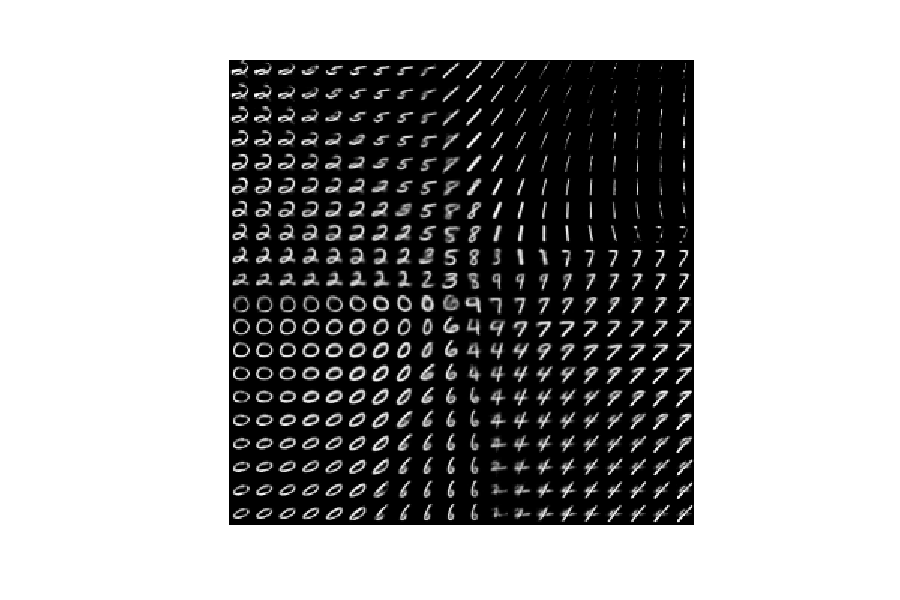
\includegraphics{media/manifold.pdf}
  \caption{MNIST 2-dimensional manifold}\label{fig:vae_manifold}
\end{figure}

\subsection{Performance}
\label{sub:vae_performance}

\subsection{Extensions}
\label{sub:vae_extensions}

\subsubsection{Deep Recurrent Attention Writer}
\label{ssub:vae_deep_recurrent_attention_writer}

\subsubsection{Importance Weighted Autoencoder \cite{iwae:2015}}
\label{ssub:vae_importance_weighted_autoencoder}

\subsubsection{Conditional VAE}
\label{ssub:vae_conditional_vae}





%----------------------------------
% Generative Adversarial Netoworks
%----------------------------------
\section{Generative Adversarial Networks}
\label{sec:gan}

%%% when introduced, game theory approach
Generative Adversarial Networks (GAN) is a framework proposed in 2014 by Goodfellow et al. \cite{gan:2014} based on a game theoretic approach to generative modelling.
%which has gathered a lot of attention in the deep learning community and in the last few years many extensions have been [proposed] (citations).

GANs circumvent the issues arising the inference problem by playing a two-player game. Both players play non-cooperatively against each other, which means they only try to maximize their respective success or profit.
One player is called the generator $G$ which tries to produce authentic looking data samples while the other player, the discrimininator $D$ has to decide whether a received sample is generated or actually real data.
It is important to note that the generator gets to know whether the discriminator accepted the generated output as \emph{real} or rejected it as \emph{fake}.

Each player plays to maximize its own success, which means the discriminator maximizes the number of samples which got discriminated correctly.
On the other side, $G$ tries to produce as many real-looking samples as possible to get accepted by $D$.\\

As the game progresses, both parties will get better at their respective objective and the generated samples will look more and more like the training examples.\\

Using the analogy of counterfeiters and police can help understand the intuition behind GANs better.
Counterfeiters will try to produce fake money looking to fool the police into thinking it is real money.
The police however is able to distinguish badly made fake money from real money easily and as such rejects the fake money with high confidence.
This rejection in turn triggers the counterfeiters to look at real money more closely and try to imitate it even better. Therefore they are able to improve the quality of the faked money. Improvements made to the fake money in this iteration will lower the confidence with which the police was able to reject previous samples.

The game-theoretic solution to the emerging situation where neither counterfeiters as generator nor police as discriminator can improve its own success with respect to the outcome of the game gets called \emph{Nash equilibrium}\cite{game_theory:1994}.

In the case of GANs, this situation means the generator produces samples which can only be rejected with probability $p=0.5$ by the discriminator, meaning it produces as good samples as there are in the dataset.\\\\

Another formulation of the GAN framework is to define the zero-sum game between the generative model and its adversary.
The payoff of the discriminator can be described as the value function $v(G,D)$ while the payoff of the generator is the negative payoff of $D$: $-v(G,D)$.\\
This formulation allows us to define the convergence as equation \ref{eq:zerosum_convergence}.
\begin{equation}
  \label{eq:zerosum_convergence}
  G^* = \arg \min_{G} \max_{D} V(G,D)
\end{equation}


% use of words: forgery
%To understand the inuition behind the approach to GANs, it may be helpful to view(?) analogy of counterfeiters and the police.
%Counterfeiters try to produce fake money imitating legit money while the police tries to distinguish fake from real money.
%This procedure of generating and distinguishing will go back-and-forth as the counterfeiters will get better at producing authentic looking money and the police is hard-pressed to differentiate between fake and real.
%Eventually, this procedure will result in a nash equlibrium where the police or discriminator will have 50\% chance of seperating authentic from real.

%Ideally, we want to find this equilibrium for the GAN model as well.




%GANs can be understood as a two-player game where one player is called generator $G$ playing against the discriminator $D$.
%The goal of $G$ is to produce similar data to the given training set while $D$ is tasked with discriminating(?) the generated samples from the training data. Both $G$ and $D$ are learning function approximators, for example Multi-Layer Peceptron (MLP) networks as proposed in the original GAN paper.
% --> declare distribution p_data, p_model, x, z
%During learning, both networks are updated in parallel according to the gradient of their respective loss function which we will explore now.\\
%In the following $p_{data}$ is the true data generating distribution from which the training samples have been generated.
%We don't have access to that distribution.


\begin{figure}[htb]
\centering
\includestandalone[width=\textwidth,mode=buildnew]{media/gan_conceptual}
  \caption{Architecture used for generative adversarial networks}
  \label{fig:gan_a}
  \medskip
  \small
  The above figure illustrates the computational graph and gradient flow in the GAN framework.\\
  $X$ denotes the dataset containing real-world samples from $p_{data}$, which we aim to model.\\
  Solid arrows indicate the forward pass in the model while dashed arrows denote the gradient flow during a backward pass.
\end{figure}

\newpage

\subsection{Architecture}
\label{sub:gan_arch}
To formalize the setting in which the game between $G$ and $D$ takes place, we define the true, however unknown data distribution $p_{data}(x)$ from which samples are available as dataset $X=\{x^{(1)}, x^{(2)}, \dots, x^{(N)}\}$.

In the case of generative modelling, the goal is to approximate $p_{data}(x)$ with $p_{model}(x)$.
GANs uses neural network as function approximator for $G$ as well as $D$.
The generator network $G$ produces samples from $p_{model}(x)$ by transforming samples from random noise as $x = G_\xi(z)$,
where $\xi$ denotes the parameters learned by the neural network representing $G$.\\
Competing with $G$ is the discriminator $D$ trained to distinguish samples $ \tilde{x} \sim p_{model}(x)$ from real data $x \sim p_{data}(x)$.\\

Figure \ref{fig:gan_a} summarizes the described architecture.\\
%Formalizing the setup in a probabilistic way, we have the unknown data distribution $p_{data}(x)$ from which the training examples have been drawn and the marginalized model distribution $p_{model}(x) = \int p(z)p(x|z) \textit{d}z$ over the noise space $z$ (also latent space).


% http://www.slideshare.net/xavigiro/deep-learning-for-computer-vision-generative-models-and-adversarial-training-upc-2016
% TODO: recreate in tikz


%\begin{figure}[htb]
%\centering
%\includestandalone[mode=buildnew,width=\linewidth]{media/gan_conceptual}
  %\caption{Conceptual idea of generative adversarial networks (source: Summer seminar UPC TelecomBCN)}\label{fig:gan_architecture}
%\end{figure}


\subsubsection{Generator Network}
The generator $G$ in the GAN framework tries to fool the discriminator $D$ by producing samples which are indistinguishable from the training data.
This process can be formally written as minimizing the following cost function.
%Where $z$ is sampling from the noise prior $p(z)$.\\

%Another common form of the generator loss is $\mathcal{L'}_g$.
%$$
\begin{equation}
  \label{eq:l_g_1}
  \mathcal{L}_g = \min \log(1 - D(G(z)))
\end{equation}

However, for gradient-based learning $\mathcal{L}_g$ provides poor gradient during learning where the discriminator is able to reject samples from the generator with high confidence.\\
Therefore is in practice often equation \ref{eq:l_g_2} instead of equation \ref{eq:l_g_1} to optimize its objective.\\
\begin{equation}
  \label{eq:l_g_2}
  \mathcal{L'}_g = \max \log D(G(z))
\end{equation}

Note that this loss function is fully differentiable which means it can be trained with backpropagation.



\subsubsection{Discriminator Network}
The objective of the discriminator network $D$ is to distinguish the generated samples produced by $G$ from the training set samples.
This process can be formalized to maximizing the cost function $\mathcal{L}_d$.
\begin{equation}
  \label{eq:l_d}
  \mathcal{L}_d = \max \log\big(\log D(x) + \log (1 - D(G(z))\big)
\end{equation}



\subsection{Training}
\label{sub:gan_training}

\begin{figure}[htb]
\centering
  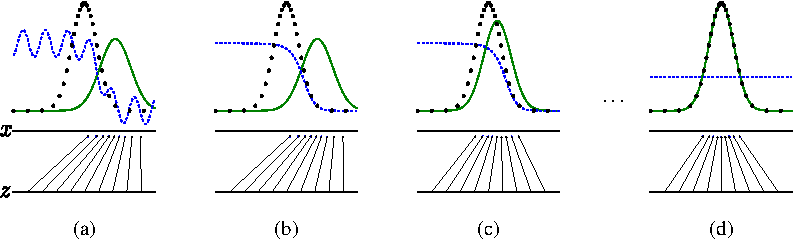
\includegraphics[width=\linewidth]{media/gan_training-crop}
  \caption{Architecture used for generative adversarial networks}
  \label{fig:gan_training}
  \medskip
  \small
\end{figure}


Combining the two objectives into one value function yields equation \ref{eq:minimax_value}.
\begin{equation}
\label{eq:minimax_value}
\min_G \max_D V(D,G) = \mathbb{E}_{x \sim p_{data}}[\log D(x)] + \mathbb{E}_{z \sim p_z(z)}[\log(1 - D(G(z)))]
\end{equation}

The GAN framework can be fully trained with stochastic backpropagation due to $V(G,D)$ being differentiable with $G$ and $D$ implemented as deep neural nets.
Figure \ref{fig:gan_training} illustrates the ideal training procedure for learning of an 1D gaussian.
Training will oscillate between training the generator and discriminator, where the other party is fixed respectively.
In order to avoid a too strong discriminator (or generator), the ratio of learning steps will vary even though there are no hard rules for this.

\vspace{5cm}
\paragraph{Theoretical Foundation}
Using a model with infinite training time and capacity in both generator and discriminator allows theoretical analysis of the GAN framework \cite{gan:2014}.
For any given generator $G$, the optimal discriminator $D$ is given by $D_G^*(x)$:
$$
D_G^*(x) = \frac{p_{data}(x)}{p_{data}(x) + p_{model}(x)}
$$

%In the original GAN paper an minibatch-based algorithm for training GAN is proposed, but we will take a look at an the online learning version below:\\
%\begin{algorithm}
  %\caption{Online learning of generative adversarial networks $-$ simple version ($k=1$)}
  %\label{alg:gan_online}
  %\begin{algorithmic}[1]
    %\Let{$\eta_d, \eta_g$}{Learning rate of discriminator and generator networks, respectively}
    %\Let{$\theta_d, \theta_g$}{Parameters of function approximators}
    %\For{number of training iterations}
      %\Let{$z_d$}{sample from noise prior $p_g(z)$}
      %\Let{$z_g$}{sample from noise prior $p_g(z)$}
      %\Let{$x$}{example from training set}
      %\Let{$\theta_d$}{$\theta_d + \eta_d \nabla_{\theta_d} \bigg[\log D(x) + \log \big(1 - D(G(z_d))\big)\bigg]$}
      %\Let{$\theta_g$}{$\theta_g - \eta_g \nabla_{\theta_g} \bigg[\log\big(1 - D(G(z_d))\big)\bigg]$}
    %\EndFor
  %\end{algorithmic}
%\end{algorithm}

%In algorithm \ref{alg:gan_online} the original algorithm has been modified for single pass (online) learning.
%Sampling minibatches from the noise prior and $p_{data}(x)$ result in the minibatch version.
%Additionally, it is often required for practical reasons to let the discriminator run multiple backward passes while updating the generator once (why?).
%Note that the discriminator will ascend while the generator descend its gradient due to maximizing $\mathcal{L}_d$ but minimizing $\mathcal{L}_g$ (correct?).

\newpage

\subsection{Stability and Performance}
\label{sub:gan_stability}
In the practical case where both function approximators $G$ and $D$ are represented using a neural network,
GANs have been shown to be difficult to train using gradient descent.
These issues have been credited to the problem of finding the nash equilibrium in the minimax-game with continious, high-dimensional parameters whereas current gradient-based methods are [designed] to reach an minimum.
Additionally to these hypothetical thoughts, \cite{gan_distinguish_crit:2014} have shown that these methods may fail to converge.
Acknoledging these problems, Salimans et al \cite{improved_gan:2016} has studied the stability and performance of GAN in detail resulting in a number of practical methods improving sample generation and improved semi-supervised learning performance.
We will take a look at a selection of these methods in the following, focussing on neural networks as approximators.

\subsubsection{Freeze Learning}
\label{ssub:gan_freeze_learning}
One of the main issues prominent during early GAN research is the disparity between $G$ and $D$.
Commonly during training one of these networks will outpace the other resulting in degraded gradients where the other player is unable to learn from.
Freeze learning is one of the natural counter to this problem, just freezing either $G$ or $D$ until the other network has catched up (formulation!).
In practice the generator is far slower to train than the discriminator in most cases (citation).


\subsubsection{Label Smoothing}
\label{ssub:gan_label_smoothing}
Another basic idea to improve gradient flow is to replace the binary classification values $0/1$ with smoothed values $0.1/0.9$ or $\epsilon/1-\epsilon$.
This guarantees to provide the generator with an informative gradient to improve learning performance
Additionally, smoothed labels have been shown to reduce the attack surface of neural networks to adversarial examples \cite{adv_examples:2016}.
% TODO replace 0/1 with e/1 − e ??
% TODO one-sided label smoothing


\subsubsection{(Virtual) Batch normalization}
\label{ssub:gan_batch_norm}
% TODO explain internal covariate shift?
Batch normalization (BN) \cite{batch_norm:2015} is a recent technique to boost performance in deep neural networks addressing the \emph{internal covariate shift} by normalizing minibatches.
Essentially, BN works by normalizing each sample from a minibatch to the statistics of the whole batch.
In a paper \cite{improved_gan:2016} by Salimans et al on improving stability of the GAN training procedure, a variant of BN has been proposed called virtual batch normalization.


%Using batch normalization \cite{batch_norm:2015} helped stabilizing learning DCGAN \cite{dcgan:2015}.
\cite{improved_gan:2016} introduced virtual batch normalization where each input $x$ is normalized on one reference batch chosen at the start of learning instead of the other inputs in the mini-batch.

\subsubsection{Feature Matching}
\label{ssub:gan_feature_matching}
In computer vision, features are often used to identify relevant pieces of information in images for recognition and classification.
They may refer to a set of points or edges in an image, which exactly is not clearly defined.
With the recent advances in classification tasks performed by deep convolutional networks, automatically learned features have been a large part of that success. (citation!)
Feature matching is an technique designed to improve the learning procedure of GANs where not directly $\mathcal{L}_g$ is maximized but instead also learn the discriminator on intermediate layer activation outputs.
Using this modified procedure the modified objective function aids the generator to output data matching the statistics of the input data.
With $f(x)$ denoting an intermediate layer in $D$, the new objective function becomes:
$$
|| \mathbb{E}_{x \sim p_{data}}f(x) - \mathbb{E}_{z \sim p(z)}f(G(z)) || ^{2}_{2}
$$




%\subsection{Application}
%\label{sub:gan_application}
%GAN have been applied to many different areas which include generating images (GAN, DCGAN, LAPGAN), sequences (SeqGAN), videos (\cite{gan_video:2016}), 3D objects (\cite{gan_3d:2016}), text-to-image synthesis (\cite{gan_t2i:2016})


\subsection{Extensions}
\label{sub:gan_extensions}

\subsubsection{DCGAN \cite{dcgan:2015}}
\label{ssub:dcgan}
Early implementations of the GAN framework have been implemented using fully-connected layers,
which have proven to be difficult and slow to train on real-world data (citation, original convnet papers?).
Using deep convolutional networks has helped reach human-level performance in object recognition and classification problems on images (citations!).
As the discriminator in the GAN model implements a binary classification task and the generator performance is heavily dependent on the discriminator, using convnets to train the model should improve performance of image generation immensely.
\emph{Deep convolutional generative adversarial network} (DCGAN) has applied convolutional networks to both generator and discriminator, resulting in quantitively evualuated better results.
DCGAN uses no fully connected or pooling layers, but instead fractionally strided convolutions (often wrongfully called deconvolutions).

\subsubsection{LAPGAN \cite{lapgan:2015}}
\label{ssub:lapgan}
LAPGAN is an extension of GAN applied to images using laplacian pyramids \cite{laplacian:1983}.
Instead of using a single generator network, LAPGAN uses a series of deep convolutional networks as generators.

\paragraph{Training} is heavily modified from the regular GAN framework.
In each iteration a training sample is drawn from the dataset and a downsamples version from it is computed.
The discriminator receives now either the computed high-pass image (from the original image and the down-then-up sampled image) or an high-pass image from the generator.
These steps are repeated for other steps, downscaling the image.
In the last stage, a traditional generator and discriminator is used for the $8x8$ image.
\paragraph{Sampling} uses a conditional GAN to produce high-resolution images through different stages of deep generator networks.

\paragraph{Results}
As GANs have no direct measurement of the quality of generations due to their lack of objective function, human evaluation of the authenticity of generated images is used for quantitive results.
LAPGAN has pushed the state of the art significantly, with generated images which are high-resolution in comparison to earlier methods and arguebly high variety of generations.
Furthermore, humans have evaluated the generated images for real images 40\% of the time.






%----------------------------------
% More Generative Directed Models
%----------------------------------
%\newpage
\section{More Generative Directed Models}
\label{sec:more}

There are several more deep directed generative models than shown here, however in order to discuss some models more in detail only two recent promising models have been presented.


\subsection{Generative Moment Matching Networks}
\label{sub:more_mmn}
Generative moment matching networks (GMMN) present a similar idea to GANs, however instead of posing the generative modelling problem as game it is optimized using \emph{maximum mean discrepancy} (MMD).

\vspace{10cm}

\subsection{Auto-Regressive Networks}
\label{sub:more_arn}

%See \cite{gan_openai:2016} and \cite{gan_training:2016}.





\newpage

\section{Summary}
\label{sec:summary}

In this article, we have taken a look at various directed models which perform generative modeling using deep neural networks.\\
After a short overview over traditional generative models and models not covered in this article, we have taken a look at a wide area of applications using generative models.\\\\
%
As one of the first basic generative models, the sigmoid belief net lays the foundation for directed generative models and displays its weaknesses during inference and training.\\
The variational autoencoders have been discussed in more detail using variational inference to turn the inference problem into an optimization problem and solving it there.
VAE and its various extensions have been shown to be a flexible tool applicable for different tasks.\\
%
Generative adversarial networks introduced in Section~\ref{sec:gan} uses a game-theoretic approach to generative modeling. In recent years, GANs have been extended of which we discussed a subset.\\\\
%
Deep generative models have shown the capability to learn rich internal representation of high-dimensional data in order to generate samples using recent advances in deep learning.
Going further, as intelligent agents will need to have accurate and generalized internal representations inferred through sensory input to reason about the world, generative models are likely to be the cornerstones of more advanced intelligent systems in the future.

%Both models explained in detail have been proposed in recent years with many proposed extensions which were not covered in this article, thus further improvements are likely to happen.

Especially interesting is the case of unsupervised learning, due to vast amount of freely available data on the web and in images, video and audio. Deep learning has been mostly focussed on supervised algorithms, however these methods require most labelled datasets which are often not feasible to obtain.

%Generative models have shown great promise to tackle interesting problems.
%Academic work is moving incredibly fast and many new ideas and combinations
%are being proposed almost daily (citation needed, meta paper?).
%For example, VAEs and GANs have been combined (https://github.com/skaae/vaeblog)
%which produced way larger images than GANs alone.

%% not relevant, but wanted to write about it :p
%As mentioned in the motivation, further advances to generative architectures are
%likely to solve current issues with depending on large labelled data.
%Another large and increasing area of research is semi-supervised learning
%(combining learning from labelled data as well as unlabelled data)
%and also one-shot learning, which is where humans excel and machines fail currently.
%\\\\
%Exciting times :)




\newpage

\addcontentsline{toc}{section}{References}
\bibliographystyle{plain}
\bibliography{paper}

\end{document}
